\documentclass[11pt,a4paper]{article}
\usepackage{xltxtra} 
\usepackage{xgreek} 
\usepackage{amsmath}
\usepackage{mathtools}
\setromanfont[Mapping=tex-text]{Kerkis}
\setmonofont[Mapping=tex-text]{Consolas}
\usepackage{hyperref} 
\raggedbottom

\newcommand{\HRule}{\rule{\linewidth}{0.5mm}}


\begin{document}

\begin{titlepage}
\centering

% Upper part of the page
%\includegraphics{Pyrforos.png}\\[1cm]    

\textsc{\LARGE Σχολή \\ Ηλεκτρολόγων Μηχανικών \\[-3pt] και \\[6pt] Μηχανικών Υπολογιστών}\\[1.5cm]
\textsc{\Large Παράλληλα Συστήματα Επεξεργασίας}\\[0.5cm]

% Title
\HRule \\[0.5cm]
{\huge \bfseries Αναφορά 2ης άσκησης}\\[0.2cm]
\HRule \\[1.5cm]

% Authors
\begin{minipage}{0.4\textwidth}
\large
Κουτσούκος Δημήτριος \\
(ΑΜ: 03110078) \\
Χαρισόπουλος Βασίλειος \\
(ΑΜ: 03110046) \\
\end{minipage}

\vfill

{\large \today}
\end{titlepage}

\clearpage
\clearpage
\newpage
\section{Παραλληλοποίηση και ζητήματα επίδοσης}
Η υλοποίηση της μεθόδου Jacobi σε αρχιτεκτονική CUDA περιορίζεται αρκετά λόγω των περιορισμών των προσβάσεων στην κύρια μνήμη.
Οι προσβάσεις στην κύρια μνήμη πριν και μετά από κάθε βήμα είναι ιδιαίτερα χρονοβόρες και περιορίζουν τον παραλληλισμό του 
αλγορίθμου. Γενικώς όταν γράφουμε κώδικα σε GPUs θα πρέπει να αποφεύγουμε τις προσβάσεις από και προς την κύρια μνήμη και αν
γίνονται τέτοιες θα πρέπει να επικαλύπτονται με υπολογισμούς για να μην χάνουμε πολύ χρόνο ή να προσπαθήσουμε να κάνουμε 
συνένωση προσβάσεων στην κύρια μνήμη. Τέλος κάθε φορά που πρέπει να συγχρονίσουμε τα threads επιβάλλεται επιπρόσθετη καθυστέρηση 
λόγω του μεγέθους αυτών στις GPUs. Λαμβάνοντας υπόψιν όλα τα παραπάνω βλέπουμε πώς για να επιτύχουμε καλή επίδοση 
που να μπορεί να συγκριθεί με άλλες τεχνικές παραλληλοποίησης όπως για παράδειγμα αυτή του openmp θα πρέπει να χρησιμοποιήσουμε
την shared memory αλλά και τεχνικές όπως το time-tiling.
\section{Υλοποίηση}
\subsection{Βασική υλοποίηση}
Στη βασική υλοποίηση κάθε thread υπολογίζει μόνο ένα στοιχείο. Πιο αναλυτικά, κάθε thread βρίσκει την θέση του στο global πίνακα που θα τρέξουμε τη μέθοδο jacobi, στη συνέχεια ελέγχει αν βρίσκεται εκτός ορίων και τέλος υπολογίζει το στοιχείο που του έχει ανατεθεί και επιστρέφει.\\  Ψάχνοντας τα specs της κάρτας γραφικών που έχουν τα termis βλέπουμε ότι έχει 1536 threads συνολικά και γνωρίζοντας ότι κάθε warp έχει 32 threads κάνοντας τη διαίρεση βλέπουμε ότι έχουμε 48 blocks δηλαδή το πολύ 8 ανά streaming multiprocessor. Προκειμένου να έχουμε πλήρη χρησιμοποίηση στα block slots πρέπει να έχουμε 
\[ \frac{1536}{8} = 192 \text{ threads per block} \] άρα το γινόμενο των διαστάσεων του block μας να είναι 192. Πειραματιζόμενοι με όλα τα γινόμενα που έχουν αυτά τα γινόμενα βρίσκουμε ότι η καλύτερη απόδοση επιτυγχάνεται για block 32x6 και είναι ίση με 28 Gflops/s. \\ Επειδή έχουμε 32 threads/warp και κάθε thread υπολογίζει μόνο ένα στοιχείο, προσπελαύνοντας στην global memory τα στοιχεία αριστερά/δεξιά και πάνω/κάτω του, το memory coalescing  επιτυγχάνεται μόνο για τα στοιχεία που βρίσκονται στην ίδια γραμμή, δηλαδή για τα αριστερά και δεξιά γειτονικά, αφού η CUDA μπορεί να συνενώσει τις προσβάσεις σε διαδοχικά στοιχεία από διαφορετικά threads σε μια μοναδική "συναλλαγή". Τέλος, με τη χρήση του CUDA Occupancy Calculator βλέπουμε ότι για αυτό που υπολογίσαμε θεωρητικά έχουμε 100\% χρησιμοποίηση της GPU.
\subsection{Χρήση της μοιραζόμενης μνήμης(shared memory)}
Με τη χρήση κοινής μνήμης κάναμε 2 υλοποιήσεις, μία "απλή" και μία πιο "σύνθετη". Στην απλή υλοποίηση χωρίζουμε ξανά τον πίνακα 
σε blocks και φορτώνουμε όλα τα στοιχεία του κάθε block στην μοιραζόμενη μνήμη και έτσι κάθε thread εντός του block μπορεί να 
προσπελάσει τα στοιχεία που χρειάζεται από την μοιραζόμενη μνήμη. Προκειμένου να μην έχουμε προβλήματα με προσβάσεις στην κύρια 
μνήμη στα εξωτερικά στοιχεία κάθε block έχει καταλαμβάνει 2 λιγότερες γραμμές και στήλες σε σχέση με τη naive υλοποίηση  και όλοι οι υπολογισμοί γίνονται σε εσωτερικούς
κόμβους. Αυτό προφανώς συνεπάγεται ότι 2 γειτονικά thread blocks θα έχουν και επικάλυψη στα εξωτερικά τους στοιχεία ώστε τελικά οι προαναφερθέντες εσωτερικοί κόμβοι να καλύπτουν ολόκληρο τον πίνακα. Κάθε thread φέρνει το αντίστοιχο στοιχείο του πίνακα, έπειτα ελέγχει αν βρίσκεται σε εξωτερικό κόμβο και στη συνέχεια αν βρίσκεται εντός του block και μετά κάνει τους
απαραίτητους υπολογισμούς. Με μία τέτοια υλοποίηση βλέπουμε ότι η απόδοση έχει μειωθεί σε σχέση με τη naive υλοποίηση και είμαστε
περίπου στα 14 Gflops/s. Η μειωμένη απόδοση καταρχάς οφείλεται στο branching που προκαλεί warp divergences και κατά δεύτερον στη 
υποχρησιμοποίηση της κάρτας γραφικών διότι τα εξωτερικά threads στο κάθε block δεν κάνουν κανένα υπολογισμό παρά μόνο φέρνουν 
στοιχεία στην μοιραζόμενη μνήμη. O παραπάνω συλλογισμός επιβεβαιώνεται και από το CUDA Occupancy Calculator. \\ \\

Στη συνέχεια τροποποιήσαμε την υλοποίηση μας προκειμένου κάθε thread να υπολογίζει παραπάνω από 1 στοιχεία. Για τη μεγιστοποίηση 
του οφέλους του memory coalescing κάθε thread φέρνει στην μοιραζόμενη μνήμη όλα τα στοιχεία αλλά υπολογίζει κατά στήλη αυτά που 
έχουμε ορίσει. Η τακτική που ακολουθούμε εδώ οφείλεται στον τρόπο που αποθηκεύονται στην Cuda τα στοιχεία της μνήμης για μια συμπαγή δομή δεδομένων όπως ένας πίνακας από 4-byte floats: συγκεκριμένα, διαδοχικά 32-bit στοιχεία αποθηκεύονται σε διαδοχικά memory banks (στην αρχιτεκτονική Fermi 32 memory banks), όπως φαίνεται στο σχήμα \ref{figure:coalescing}.
\begin{figure}[h]
	\centering
	\includegraphics[scale=0.8]{coalescing_cuda.eps} 
	\caption{Αποθήκευση διαδοχικών στοιχείων σε memory banks}	
	\label{figure:coalescing}
\end{figure} 
(Στο σχήμα έχει υποτεθεί ότι $n < 32$). \\
Έτσι 32 threads μπορούν να προσπελάσουν ισάριθμα διαφορετικά στοιχεία, αρκεί το καθένα από αυτά να βρίσκεται σε διαφορετικό memory bank. Έτσι, εάν στην shared memory μια ομάδα από threads προσπελαύνει ισάριθμα διαδοχικά στοιχεία, εκμεταλλευόμαστε τα memory banks μεγιστοτρόπως. Με το να αναθέτουμε σε κάθε thread να υπολογίζει στοιχεία ανά στήλη, εξασφαλίζουμε ότι σε κάθε φάση της εκτέλεσης η ομάδα αυτών των threads θα προσπελαύνει στοιχεία της ίδιας γραμμής. Αντίθετα αν ένα thread υπολόγιζε διαδοχικά στοιχεία της γραμμής, θα αυξανόταν τα bank conflicts αφού πολλά threads πιθανώς να προσπαθούσαν να προσπελάσουν στοιχεία που απέχουν μεταξύ τους τέτοιο offset ώστε να βρίσκονται στο ίδιο memory bank. \\
Σε όλες τις υλοποιήσεις πέρα από τη naive χρειάζεται συγχρονισμός των 
threads αφού γίνει η μεταφορά των απαιτούμενων στοιχείων από την κύρια μνήμη στη μοιραζόμενη μνήμη. Βλέπουμε ότι όντως βελτιώνεται
η απόδοση σε σχέση με την απλή shared memory κάτι που οφείλεται στο υπάρχουν παράλληλοι υπολογισμοί διπλανών threads και μεταφορές 
στοιχείων που επικαλύπτονται με αυτούς τους υπολογισμούς. Βλέπουμε ότι συγκρινόμενο με το OpenMp η επίδοσή του είναι πολύ καλύτερη διότι
η μέγιστη επίδοση που επιτυγχάνεται στο πρώτο είναι 23 Gflops/s ενώ στο δεύτερο 9.78 Gflops/s. To Occupancy Calculator υπολογίζει τη
χρησιμοποίηση της κάρτας στο μέγιστο δυνατό βαθμό.
\subsection{Time-tiled υλοποίηση}
Σε αυτή την υλοποίηση κάθε thread block πρέπει να διαχειρίζεται διαφορετικά τα στοιχεία σε κάθε στρώμα της halo περιοχής. Τα στοιχεία που βρίσκονται
στο εξωτερικό της μεταφέρονται στη μοιραζόμενη μνήμη χωρίς να πραγματοποιούνται σε αυτά επιπλέον υπολογισμοί. Για τα στοιχεία που βρίσκονται στο 
εσωτερικό της, απαιτείται επιπλέον έλεγχος ορίων για να μην γίνονται υπολογισμοί σε περίπτωση που αυτά αντιστοιχούν σε στοιχεία του εξωτερικού του 
πίνακα που έχουν σταθερή τιμή. Μετά τον υπολογισμο όλων των τιμών(όχι μόνο αυτών της halo περιοχής) για T-1 χρονικά βήματα απαιτείται επιπλέον έλεγχος
ορίων ώστε να μην αντιγραφούν στον κύριο πίνακα οι τιμές της halo περιοχής. \\ \\
Μια σημαντική παρατήρηση εδώ είναι ότι ο έλεγχος περιοχής για τα στοιχεία που διαχειρίζεται ένα thread μπορεί να γίνει στην αρχική φάση του prefetching των στοιχείων από την κύρια μνήμη και το αποτέλεσμα να αποθηκευθεί σε έναν boolean πίνακα, ώστε να μην γίνεται από την αρχή σε καθεμία από τις φάσεις που χρειάζεται (π.χ. για τα $T - 1$ χρονικά βήματα που προηγούνται της τελικής φάσης των υπολογισμών). Πράγματι η υλοποίηση αυτής της μορφής "vectored" checking βελτίωσε αισθητά την απόδοση μας κατά το στάδιο του πειραματισμού. \\ \\
Σχετικά με το ζήτημα του αριθμού των απαιτούμενων πυρήνων για την επίτευξη μιας αποδοτικής υλοποίησης, φαίνεται πως δεν υπάρχει κάποιο άμεσα ορατό όφελος από την διάσπαση των υπολογισμών που απαιτεί ο time-tiled τρόπος σε διαφορετικούς πυρήνες. Ένα επιπρόσθετο κόστος που θα επέφερε αυτό είναι προφανώς το κόστος του kernel launching. Ακόμη, ανάλογα την υλοποίηση πιθανώς να είχαμε μεγαλύτερο branching ή μεγαλύτερο κόστος μεταφοράς στοιχείων. Έτσι, για μία αποδοτική υλοποίηση φαίνεται πως απαιτείται ένας πυρήνας αφού πειραματιζόμενοι με τις παραμέτρους της time-tiled υλοποίηση πετυχαίνουμε απόδοση 45 Gflops/s, που είναι περίπου διπλάσια από την 
shared memory και τουλάχιστον $1.5$  φορά πάνω από τη naive υλοποίηση. Σε σύγκριση δε με το OpenMp βλέπουμε ότι η απόδοση έχει αύξηση 450\%. Άλλωστε, με χρήση του CUDA Occupancy Calculator βλέπουμε ότι για τις παραμέτρους που επιλέξαμε έχουμε χρησιμοποίηση της κάρτας στο 100\%. Οι παράμετροι αυτές είναι: 
\begin{itemize}
	\item Block Size X = $96 (= 88 + 2 * T) $ 
	\item Block Size Y = $8 \left( = 6 + 2 \frac{T}{\text{elems per thread}}\right) $
	\item $ T = 4 $
	\item elements per thread = $4$
\end{itemize}
\newpage
\section{Αποτελέσματα μετρήσεων - Επιδόσεις προγραμμάτων}
Στη συνέχεια παρουσιάζονται συγκριτικά τα αποτελέσματα των μετρήσεων που πήραμε για τις διάφορες εκδοχές της Jacobi. Η μετρική που χρησιμοποιήσαμε ήταν τα Gflops, δηλαδή το πλήθος πράξεων κινητής υποδιαστολής ανά δευτερόλεπτο. \\
\begin{figure}[h]
	\centering
	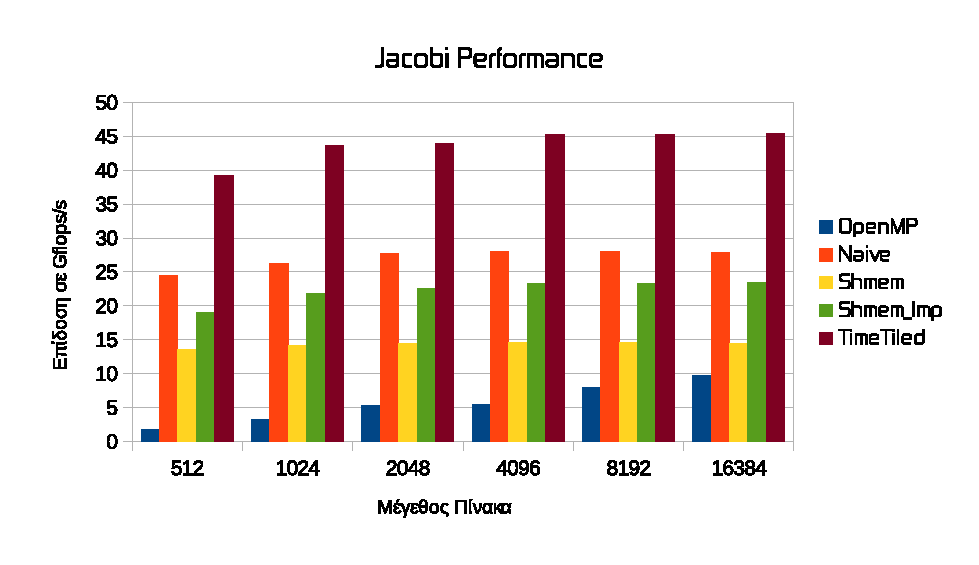
\includegraphics[width=\textwidth]{jacobi.eps}
	\caption{Απόδοση του υπολογιστικού πυρήνα}
\end{figure} \\
Όπως φαίνεται η naive φαίνεται να είναι η δεύτερη καλύτερη υλοποίηση μετά την time-tiled ενώ ακολουθεί η βελτιωμένη shared memory έκδοση. Όλες οι υλοποιήσεις (πλην της open mp) παρουσιάζουν σχετικά σταθερή απόδοση από ένα μέγεθος πίνακα κι έπειτα, κάτι που είναι λογικό αφού το πλήθος των threads είναι μικρότερο από το πλήθος των στοιχείων και επομένως δεν υπάρχει κάποια υπόνοια underutilization της συσκευής (έπειτα και από την θεωρητική επιβεβαίωση της μεγιστοβάθμιας εκμετάλλευσης της κάρτας μέσω του occupancy calculator) από τις υλοποιήσεις μας σε σχέση με τα μεγέθη του πίνακα. Αντίθετα, η υλοποίηση σε open mp παρουσιάζει υπογραμμικό scaling, ωστόσο η τελική επίδοση είναι περίπου 10 Gflops και απογοητευτική συγκριτικά με τα 45 Gflops της time-tiled υλοποίησης. \\ \\
Μια ακόμα παρατήρηση που μπορούμε να κάνουμε είναι ότι ο υπολογιστικός πυρήνας της μεθόδου jacobi ακολουθεί τέτοιο μοτίβο υπολογισμών και προσβάσεων στη μνήμη ώστε να επιτρέπει μια πάρα πολύ απλή υλοποίηση στο περιβάλλον της CUDA η οποία να είναι και αποδοτική, όπως φαίνεται από την επίδοση της naive έκδοσης της jacobi. Πιο σύνθετοι υπολογιστικοί πυρήνες πιθανώς να ευνοούν πολύ περισσότερο την προσεκτική σχεδίαση μιας υλοποίησης που να εκμεταλλεύεται έντονα το memory coalescing και την μοιραζόμενη μνήμη των thread blocks - χωρίς ωστόσο να υποτιμούμε την εντυπωσιακή βελτίωση που μας προσέφερε η time-tiled υλοποίηση. \\
Στη συνέχεια φαίνονται και οι συνολικές επιδόσεις των προγραμμάτων, που περιλαμβάνουν και τον απαιτούμενο χρόνο μεταφοράς των στοιχείων. \\
\begin{figure}[h]
	\centering
	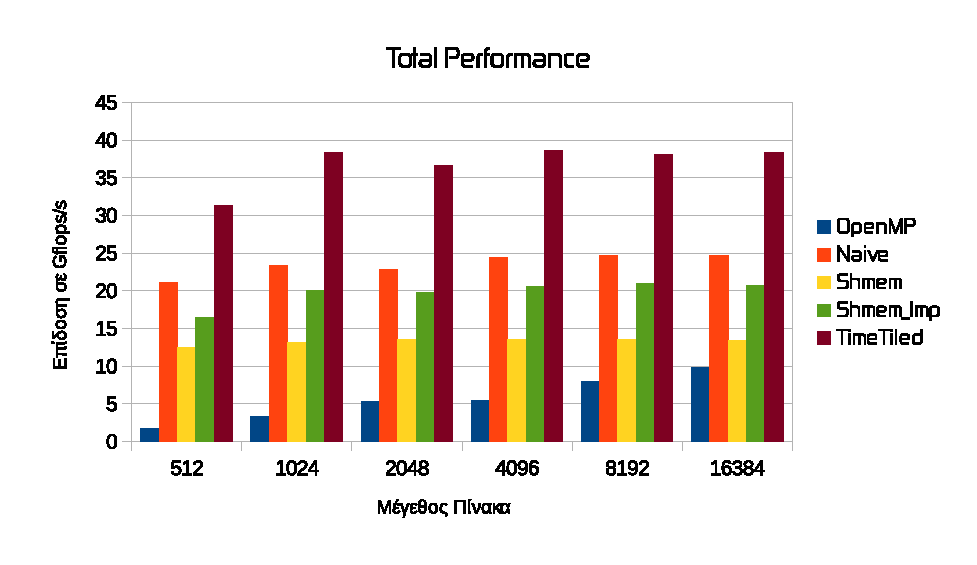
\includegraphics[width=\textwidth]{total.eps}
	\caption{Απόδοση του συνολικού προγράμματος}
\end{figure} \\
Όπως γίνεται αντιληπτό, οι υλοποιήσεις σε CUDA παρουσιάζουν μια απόκλιση λίγων Gflops (από 2-3 έως και 7) της επίδοσης του υπολογιστικού πυρήνα από την συνολική επίδοση. H μείωση αυτή οφείλεται προφανώς στον χρόνο που απαιτείται για την αντιγραφή των στοιχείων από και προς την κάρτα γραφικών, χρόνος ο οποίος δεν είναι αμελητέος για μεγάλα μεγέθη πινάκων. Αντίθετα η υλοποίηση σε OpenMP δεν παρουσιάζει καμία μείωση αφού δεν απαιτείται και καμία μεταφορά δεδομένων. \\
Συνολικά, παρά τη μείωση αυτή η επίλυση του προβλήματος της διάδοσης θερμότητας φαίνεται να ευνοεί την λύση του cuda programming αφού ακόμα και με αυτήν οι επιδόσεις είναι πολύ καλύτερες.

\newpage

\section*{Αναφορές - Βιβλιογραφία}
\begin{enumerate}
\item 
\href{http://docs.nvidia.com/cuda/cuda-c-programming-guide/}{The Cuda C Programming Guide}
\item  \href{http://devblogs.nvidia.com/parallelforall/how-access-global-memory-efficiently-cuda-c-kernels/}{How to access global memory efficiently in CUDA C Kernels}
\item 
\href{http://devblogs.nvidia.com/parallelforall/using-shared-memory-cuda-cc/}{Using Shared Memory in CUDA C}
\item
\href{http://www.cslab.ece.ntua.gr/courses/pps/files/fall2014/CUDApresentation-Fall2014.pdf}{Παράλληλος Προγραμματισμός σε Επεξεργαστές Γραφικών}
\end{enumerate}

\end{document}
